\chapter{Complex Analysis}

Complex analysis studies functions of a complex variable. At first glance, it may look like ordinary calculus performed on the complex plane. However, this impression is misleading. Complex differentiability is far more rigid than real differentiability. A function that is differentiable once in the complex sense is automatically infinitely differentiable and locally represented by a power series. This is one of the most beautiful phenomena in mathematics.

The central reason is that complex numbers contain both algebraic and geometric information. Multiplication by a complex number combines scaling and rotation. Therefore, a complex derivative is not merely a rate of change; it is a local similarity transformation. This geometric constraint forces complex differentiable functions to have strong structure.

This chapter develops the basic route of complex analysis:
\[
    \text{complex numbers}\to\text{complex differentiability}\to\text{Cauchy theory}\to\text{power series}\to\text{residues}.
\]

\section{Complex Numbers and the Complex Plane}


The complex plane should be read simultaneously as an algebraic field and as a geometric plane. Addition corresponds to vector translation, while multiplication corresponds to scaling and rotation. This dual interpretation is the reason complex numbers are so efficient in geometry, differential equations, Fourier analysis, and signal processing. They package two real coordinates into one object whose arithmetic remembers planar geometry.

Whenever possible, it is useful to translate a complex formula into a geometric statement. The modulus $|z|$ is distance from the origin, $|z-w|$ is distance between points, conjugation reflects across the real axis, and multiplication by $e^{i\theta}$ rotates through angle $\theta$. These interpretations make later ideas such as conformality and residues much less mysterious.

\subsection{Algebraic Definition}

\begin{definition}[Complex Numbers]
The set of complex numbers is
\[
    \mathbb{C}=\{a+bi:a,b\in\mathbb{R},\ i^2=-1\}.
\]
For $z=a+bi$, the real and imaginary parts are
\[
    \operatorname{Re}z=a,
    \qquad
    \operatorname{Im}z=b.
\]
\end{definition}

Addition and multiplication are defined by the rules
\[
    (a+bi)+(c+di)=(a+c)+(b+d)i,
\]
and
\[
    (a+bi)(c+di)=(ac-bd)+(ad+bc)i.
\]

\begin{definition}[Complex Conjugate and Modulus]
For $z=a+bi\in\mathbb{C}$, define its \textbf{complex conjugate} by
\[
    \overline{z}=a-bi,
\]
and its \textbf{modulus} by
\[
    |z|=\sqrt{a^2+b^2}.
\]
\end{definition}

\begin{proposition}[Basic Identities]
For $z,w\in\mathbb{C}$,
\begin{enumerate}
    \item $z\overline{z}=|z|^2$;
    \item $\overline{z+w}=\overline{z}+\overline{w}$;
    \item $\overline{zw}=\overline{z}\,\overline{w}$;
    \item $|zw|=|z||w|$;
    \item if $z\neq 0$, then $z^{-1}=\overline{z}/|z|^2$.
\end{enumerate}
\end{proposition}

\begin{proof}
Each identity follows directly from writing $z=a+bi$ and $w=c+di$. For example,
\[
    z\overline{z}=(a+bi)(a-bi)=a^2+b^2=|z|^2.
\]
If $z\neq 0$, then
\[
    z\frac{\overline{z}}{|z|^2}=\frac{z\overline{z}}{|z|^2}=1.
\]
\end{proof}

\subsection{Geometric Interpretation}

A complex number $z=a+bi$ can be viewed as the point $(a,b)$ in the plane. Under this identification, addition of complex numbers is vector addition.

Multiplication has a richer meaning. If $z$ has modulus $r$ and argument $\theta$, then multiplication by $z$ scales lengths by $r$ and rotates angles by $\theta$.

\begin{definition}[Argument]
For a non-zero complex number $z=a+bi$, an \textbf{argument} of $z$ is any real number $\theta$ such that
\[
    a=|z|\cos\theta,
    \qquad
    b=|z|\sin\theta.
\]
The set of all arguments differs by integer multiples of $2\pi$.
\end{definition}

\begin{definition}[Polar Form]
Every non-zero complex number can be written as
\[
    z=r(\cos\theta+i\sin\theta),
\]
where $r=|z|>0$ and $\theta$ is an argument of $z$.
\end{definition}

\subsection{Euler's Formula}


Euler's formula is more than a memorable identity; it is the bridge between exponential growth and circular motion. In real analysis, the exponential function and trigonometric functions appear to describe different phenomena. In complex analysis they become different shadows of the same function. This unification is one reason complex methods simplify oscillatory problems.

The formula also explains why polar form is natural. Writing $z=re^{i\theta}$ separates size from direction. Multiplication then becomes especially transparent: sizes multiply and angles add. This is often the simplest way to compute powers, roots, and rotations.

\begin{theorem}[Euler's Formula]
For every real number $\theta$,
\[
    e^{i\theta}=\cos\theta+i\sin\theta.
\]
\end{theorem}

\begin{proof}[Proof via Taylor Series]
Using the Taylor series expansions,
\[
    e^x=\sum_{n=0}^{\infty}\frac{x^n}{n!},
    \qquad
    \cos x=\sum_{n=0}^{\infty}(-1)^n\frac{x^{2n}}{(2n)!},
    \qquad
    \sin x=\sum_{n=0}^{\infty}(-1)^n\frac{x^{2n+1}}{(2n+1)!},
\]
we substitute $x=i\theta$:
\[
    e^{i\theta}=1+i\theta-\frac{\theta^2}{2!}-i\frac{\theta^3}{3!}+\frac{\theta^4}{4!}+\cdots.
\]
Grouping real and imaginary parts gives
\[
    e^{i\theta}=\left(1-\frac{\theta^2}{2!}+\frac{\theta^4}{4!}-\cdots\right)
    +i\left(\theta-\frac{\theta^3}{3!}+\frac{\theta^5}{5!}-\cdots\right),
\]
which equals $\cos\theta+i\sin\theta$.
\end{proof}

\begin{corollary}[Exponential Form]
Every non-zero complex number can be written as
\[
    z=re^{i\theta},
\]
where $r=|z|$ and $\theta$ is an argument of $z$.
\end{corollary}

\begin{proposition}[Multiplication in Polar Form]
If
\[
    z_1=r_1e^{i\theta_1},
    \qquad
    z_2=r_2e^{i\theta_2},
\]
then
\[
    z_1z_2=r_1r_2e^{i(\theta_1+\theta_2)}.
\]
\end{proposition}

\begin{proof}
Using laws of exponentials,
\[
    z_1z_2=r_1r_2e^{i\theta_1}e^{i\theta_2}=r_1r_2e^{i(\theta_1+\theta_2)}.
\]
\end{proof}

\begin{theorem}[De Moivre's Formula]
For $n\in\mathbb{Z}$,
\[
    (\cos\theta+i\sin\theta)^n=\cos(n\theta)+i\sin(n\theta).
\]
\end{theorem}

\begin{proof}
Since $\cos\theta+i\sin\theta=e^{i\theta}$,
\[
    (\cos\theta+i\sin\theta)^n=(e^{i\theta})^n=e^{in\theta}=\cos(n\theta)+i\sin(n\theta).
\]
\end{proof}

\begin{example}[Roots of Unity]
The solutions of $z^n=1$ are
\[
    z_k=e^{2\pi i k/n},\qquad k=0,1,\dots,n-1.
\]
Geometrically, these are the vertices of a regular $n$-gon on the unit circle.
\end{example}

\section{Topology of the Complex Plane}


The topology of the complex plane is the stage on which complex functions live. Open sets matter because complex differentiability is defined only at points with room to move in every nearby direction. If the domain were not open, the difference quotient might be forced to approach along only part of the plane, which would not capture genuine complex differentiability.

Domains are required to be connected because many central theorems depend on the ability to move from one point to another without leaving the region. The identity theorem, for example, uses connectedness to propagate equality from a small neighborhood to the whole domain. Without connectedness, a holomorphic function could behave independently on different components.

Since $\mathbb{C}$ is identified with $\mathbb{R}^2$, it inherits the usual topology from the Euclidean plane.

\begin{definition}[Open Disk]
For $z_0\in\mathbb{C}$ and $r>0$, the open disk centered at $z_0$ with radius $r$ is
\[
    D(z_0,r)=\{z\in\mathbb{C}:|z-z_0|<r\}.
\]
\end{definition}

\begin{definition}[Domain]
A subset $\Omega\subseteq\mathbb{C}$ is called a \textbf{domain} if it is open and connected.
\end{definition}

\begin{definition}[Limit and Continuity]
Let $f:\Omega\to\mathbb{C}$ and let $z_0$ be a limit point of $\Omega$. We say
\[
    \lim_{z\to z_0}f(z)=L
\]
if for every $\varepsilon>0$, there exists $\delta>0$ such that
\[
    0<|z-z_0|<\delta
    \quad\Longrightarrow\quad
    |f(z)-L|<\varepsilon.
\]
The function $f$ is continuous at $z_0$ if $\lim_{z\to z_0}f(z)=f(z_0)$.
\end{definition}

The definition is formally identical to the real-variable definition, but there is a crucial difference: $z$ can approach $z_0$ from infinitely many directions in the plane.

\section{Complex Differentiability}


The decisive point in complex differentiability is that the difference quotient must have a single limit no matter how $h$ approaches zero. In real one-variable calculus there are only two basic directions of approach, left and right. In the complex plane there are infinitely many directions, and they must all agree. This requirement forces the derivative to behave like multiplication by one complex number.

Thus complex differentiability is much stronger than differentiability of the real and imaginary parts as functions of two real variables. A general real differentiable map from $\mathbb{R}^2$ to $\mathbb{R}^2$ can stretch in different directions, shear, or distort angles. A complex derivative, when non-zero, can only scale and rotate infinitesimally. This geometric rigidity is the source of most powerful theorems in the subject.

\subsection{Definition of Complex Derivative}

\begin{definition}[Complex Derivative]
Let $\Omega\subseteq\mathbb{C}$ be open and let $f:\Omega\to\mathbb{C}$. We say $f$ is \textbf{complex differentiable} at $z_0\in\Omega$ if the limit
\[
    f'(z_0)=\lim_{h\to 0}\frac{f(z_0+h)-f(z_0)}{h}
\]
exists as a complex number.
\end{definition}

This looks like the usual derivative, but $h$ approaches $0$ through the complex plane. The quotient must approach the same limit along every direction.

\begin{example}
The function $f(z)=z^2$ is complex differentiable everywhere, and
\[
    f'(z)=2z.
\]
Indeed,
\[
    \frac{(z+h)^2-z^2}{h}=2z+h\to 2z.
\]
\end{example}

\begin{example}[Complex Conjugation]
The function $f(z)=\overline{z}$ is not complex differentiable at any point. At $z_0$,
\[
    \frac{\overline{z_0+h}-\overline{z_0}}{h}=\frac{\overline{h}}{h}.
\]
If $h$ is real, this quotient is $1$. If $h=it$ with $t\in\mathbb{R}$, then $\overline{h}/h=(-it)/(it)=-1$. The limit depends on direction, so it does not exist.
\end{example}

\subsection{Holomorphic Functions}


The word ``holomorphic'' should be read as a local condition. A function is holomorphic on a region if every point of the region has a neighborhood where the complex derivative exists. This local definition is deceptively modest: after Cauchy's theorem is established, holomorphicity implies integral formulas, power series expansions, and strong global restrictions.

It is also useful to distinguish being complex differentiable at a single point from being holomorphic on an open set. A function may satisfy the Cauchy-Riemann equations at one isolated point for accidental reasons. Holomorphicity requires stable differentiability throughout a neighborhood, and that stability is what unlocks the full theory.

\begin{definition}[Holomorphic Function]
Let $\Omega\subseteq\mathbb{C}$ be open. A function $f:\Omega\to\mathbb{C}$ is \textbf{holomorphic} on $\Omega$ if it is complex differentiable at every point of $\Omega$.
\end{definition}

Some authors use the word \textbf{analytic} to mean locally representable by a power series. A major theorem of complex analysis states that holomorphic and analytic are equivalent.

\begin{proposition}[Rules of Differentiation]
If $f$ and $g$ are complex differentiable at $z_0$, then:
\begin{enumerate}
    \item $(f+g)'(z_0)=f'(z_0)+g'(z_0)$;
    \item $(fg)'(z_0)=f'(z_0)g(z_0)+f(z_0)g'(z_0)$;
    \item if $g(z_0)\neq 0$, then
    \[
        \left(\frac{f}{g}\right)'(z_0)=\frac{f'(z_0)g(z_0)-f(z_0)g'(z_0)}{g(z_0)^2};
    \]
    \item the chain rule holds: $(g\circ f)'(z_0)=g'(f(z_0))f'(z_0)$.
\end{enumerate}
\end{proposition}

\section{Cauchy-Riemann Equations}


The Cauchy-Riemann equations express the compatibility between real two-dimensional differentiability and complex multiplication. If the real Jacobian matrix of $f=u+iv$ is to represent multiplication by a complex number $a+bi$, it must have the special form
\[
    \begin{pmatrix}
        a & -b\\
        b & a
    \end{pmatrix}.
\]
The equations $u_x=v_y$ and $u_y=-v_x$ are exactly the statement that the Jacobian has this form.

This matrix viewpoint is often the fastest way to remember the equations. The derivative of a holomorphic function is not an arbitrary linear transformation of the plane. It is a similarity transformation: a uniform scaling combined with a rotation. The Cauchy-Riemann equations are the coordinate expression of that fact.

Let
\[
    f(z)=u(x,y)+iv(x,y),
    \qquad z=x+iy,
\]
where $u,v:\Omega\subseteq\mathbb{R}^2\to\mathbb{R}$.

If $f$ is complex differentiable at $z_0=x_0+iy_0$, then the limit defining $f'(z_0)$ must be the same along the real and imaginary directions.

Along the real direction, $h\in\mathbb{R}$:
\[
    f'(z_0)=u_x(x_0,y_0)+iv_x(x_0,y_0).
\]
Along the imaginary direction, $h=it$:
\[
    f'(z_0)=\frac{u(x_0,y_0+t)-u(x_0,y_0)+i(v(x_0,y_0+t)-v(x_0,y_0))}{it}.
\]
Since division by $i$ equals multiplication by $-i$, this gives
\[
    f'(z_0)=v_y(x_0,y_0)-iu_y(x_0,y_0).
\]
Equating real and imaginary parts yields the Cauchy-Riemann equations.

\begin{theorem}[Cauchy-Riemann Equations]
If $f=u+iv$ is complex differentiable at $z_0=x_0+iy_0$ and the relevant partial derivatives exist, then
\[
    u_x=v_y,
    \qquad
    u_y=-v_x
\]
at $(x_0,y_0)$.
\end{theorem}

\begin{theorem}[Sufficient Condition]
Let $f=u+iv$ be defined on an open set $\Omega$. If $u$ and $v$ have continuous first partial derivatives and satisfy the Cauchy-Riemann equations on $\Omega$, then $f$ is holomorphic on $\Omega$.
\end{theorem}

\begin{example}
For $f(z)=z^2$, we have
\[
    z^2=(x+iy)^2=x^2-y^2+i(2xy).
\]
Thus $u=x^2-y^2$ and $v=2xy$. Then
\[
    u_x=2x=v_y,
    \qquad
    u_y=-2y=-v_x.
\]
The Cauchy-Riemann equations hold everywhere.
\end{example}

\begin{example}
For $f(z)=\overline{z}=x-iy$, we have $u=x$ and $v=-y$. Then
\[
    u_x=1,
    \qquad
    v_y=-1.
\]
The first Cauchy-Riemann equation fails everywhere, so $f$ is not holomorphic.
\end{example}

\subsection{Geometric Meaning}

If $f'(z_0)\neq 0$, then near $z_0$,
\[
    f(z_0+h)\approx f(z_0)+f'(z_0)h.
\]
Multiplication by $f'(z_0)$ scales and rotates small vectors. Therefore holomorphic functions with non-zero derivative preserve angles locally. Such maps are called conformal.

\begin{definition}[Conformal Map]
A holomorphic function $f$ is \textbf{conformal} at $z_0$ if $f'(z_0)\neq 0$. It is conformal on a domain if it is conformal at every point of that domain.
\end{definition}

\section{Elementary Holomorphic Functions}


Elementary functions in complex analysis are not merely copied from real analysis. They are usually defined by power series or by algebraic combinations of the complex exponential, because these definitions automatically produce holomorphic functions and preserve the identities that matter most. Once defined this way, the functions often reveal behavior impossible in the real setting.

For instance, complex sine and cosine are no longer bounded. The exponential function is periodic in the imaginary direction because $e^{z+2\pi i}=e^z$. These facts are not exceptions; they are consequences of extending real functions into a two-dimensional algebraic setting.

\subsection{Exponential and Trigonometric Functions}

\begin{definition}[Complex Exponential]
For $z\in\mathbb{C}$, define
\[
    e^z=\sum_{n=0}^{\infty}\frac{z^n}{n!}.
\]
\end{definition}

This series converges for all $z\in\mathbb{C}$ and defines an entire function.

\begin{proposition}
The complex exponential satisfies
\[
    (e^z)'=e^z,
    \qquad
    e^{z+w}=e^ze^w.
\]
\end{proposition}

\begin{definition}[Complex Sine and Cosine]
Define
\[
    \cos z=\frac{e^{iz}+e^{-iz}}{2},
    \qquad
    \sin z=\frac{e^{iz}-e^{-iz}}{2i}.
\]
\end{definition}

\begin{proposition}
For all $z\in\mathbb{C}$,
\[
    \frac{d}{dz}\sin z=\cos z,
    \qquad
    \frac{d}{dz}\cos z=-\sin z.
\]
\end{proposition}

\subsection{Complex Logarithm}


The logarithm is the first place where topology visibly enters complex analysis. Locally, away from the origin and away from a chosen branch cut, one can choose a continuous argument and define a single-valued logarithm. Globally on $\mathbb{C}\setminus\{0\}$ this is impossible because a loop around the origin changes the argument by $2\pi$.

This failure is not an algebraic inconvenience but a topological obstruction. The punctured plane has a hole, and the argument records how many times a path winds around that hole. Later, residues and contour integrals will turn this winding behavior into exact numerical invariants.

The logarithm is more subtle in complex analysis because the argument is multi-valued.

If $z=re^{i\theta}$, then a logarithm of $z$ should satisfy
\[
    e^w=z.
\]
Writing $w=u+iv$, this gives $e^u=r$ and $v=\theta+2\pi k$.

\begin{definition}[Multi-valued Logarithm]
For $z\neq 0$, the complex logarithm is the multi-valued expression
\[
    \log z=\ln|z|+i(\arg z+2\pi k),\qquad k\in\mathbb{Z}.
\]
\end{definition}

\begin{definition}[Principal Branch]
The \textbf{principal argument} $\operatorname{Arg}z$ is chosen in $(-\pi,\pi]$. The corresponding principal logarithm is
\[
    \operatorname{Log}z=\ln|z|+i\operatorname{Arg}z.
\]
It is defined on $\mathbb{C}\setminus(-\infty,0]$ if one wants a continuous single-valued branch.
\end{definition}

\begin{remark}
The impossibility of defining a continuous single-valued logarithm on all of $\mathbb{C}\setminus\{0\}$ is topological. Going once around the origin changes the argument by $2\pi$.
\end{remark}

\section{Complex Integration}


A contour integral is a line integral written in complex notation. The path supplies the direction of motion through the factor $\gamma'(t)$, while the function supplies the complex value being accumulated. Because complex multiplication contains rotation, the integral is sensitive not only to the values of $f$ but also to the orientation and winding of the path.

The example $\int_{|z|=1}1/z\,dz=2\pi i$ should be treated as a warning sign. In ordinary real calculus, a derivative with an antiderivative integrates to zero around closed loops. Here $1/z$ is locally the derivative of a logarithm, but no global single-valued logarithm exists on the punctured plane. The non-zero integral detects this global obstruction.

\subsection{Curves and Contour Integrals}

\begin{definition}[Path]
A \textbf{path} in $\mathbb{C}$ is a continuous function
\[
    \gamma:[a,b]\to\mathbb{C}.
\]
If $\gamma$ is continuously differentiable except possibly at finitely many points, it is called a \textbf{piecewise smooth path}.
\end{definition}

\begin{definition}[Contour Integral]
Let $f$ be continuous on a set containing the image of a piecewise smooth path $\gamma:[a,b]\to\mathbb{C}$. The \textbf{contour integral} of $f$ along $\gamma$ is
\[
    \int_\gamma f(z)\,dz=\int_a^b f(\gamma(t))\gamma'(t)\,dt.
\]
\end{definition}

\begin{example}
Let $\gamma(t)=e^{it}$, $0\leq t\leq 2\pi$, be the unit circle traversed counterclockwise. Then
\[
    \int_\gamma \frac{1}{z}\,dz
    =\int_0^{2\pi}\frac{1}{e^{it}}ie^{it}\,dt
    =\int_0^{2\pi} i\,dt
    =2\pi i.
\]
This example is fundamental: $1/z$ has no global primitive on $\mathbb{C}\setminus\{0\}$.
\end{example}

\begin{proposition}[Estimation Lemma]
If $|f(z)|\leq M$ on a path $\gamma$ of length $L$, then
\[
    \left|\int_\gamma f(z)\,dz\right|\leq ML.
\]
\end{proposition}

\begin{proof}
By the definition of contour integral,
\[
    \left|\int_\gamma f(z)\,dz\right|
    \leq \int_a^b |f(\gamma(t))||\gamma'(t)|\,dt
    \leq M\int_a^b|\gamma'(t)|\,dt=ML.
\]
\end{proof}

\subsection{Primitives}

\begin{definition}[Primitive]
Let $f$ be holomorphic on a domain $\Omega$. A function $F$ is a \textbf{primitive} of $f$ on $\Omega$ if $F'=f$ on $\Omega$.
\end{definition}

\begin{theorem}[Fundamental Theorem for Complex Line Integrals]
If $F'=f$ on a domain containing a path $\gamma$ from $a$ to $b$, then
\[
    \int_\gamma f(z)\,dz=F(b)-F(a).
\]
In particular, the integral of $f$ around any closed path is $0$.
\end{theorem}

\begin{proof}
Using the definition of contour integral and the chain rule,
\[
    \int_\gamma f(z)\,dz=\int_\alpha^\beta f(\gamma(t))\gamma'(t)\,dt
    =\int_\alpha^\beta (F\circ\gamma)'(t)\,dt=F(\gamma(\beta))-F(\gamma(\alpha)).
\]
\end{proof}

\section{Cauchy's Theorem and Cauchy's Integral Formula}


Cauchy's theorem says that holomorphic functions have path-independent integrals on simply connected domains. Conceptually, holomorphicity is a local condition, while simple connectedness removes global holes. When both are present, closed contour integrals vanish. If a hole is present, the local condition may still hold but a contour can wind around the hole and produce a non-zero integral.

Cauchy's integral formula is even stronger. It says that the value of a holomorphic function at an interior point is determined by its values on a surrounding circle. This is a profound difference from real analysis: holomorphic functions cannot be freely modified at one point without affecting their behavior elsewhere. Boundary data controls interior data.

The Cauchy theory is the core of elementary complex analysis. It explains why holomorphic functions are rigid.

\begin{theorem}[Cauchy's Theorem, Simple Form]
Let $\Omega$ be a simply connected domain and let $f$ be holomorphic on $\Omega$. Then for every closed piecewise smooth path $\gamma$ in $\Omega$,
\[
    \int_\gamma f(z)\,dz=0.
\]
\end{theorem}

\begin{remark}
The condition that $\Omega$ is simply connected cannot be omitted. The function $1/z$ is holomorphic on $\mathbb{C}\setminus\{0\}$, but its integral around the unit circle is $2\pi i$.
\end{remark}

\begin{theorem}[Cauchy's Integral Formula]
Let $f$ be holomorphic on an open set containing the closed disk $\overline{D(z_0,R)}$. If $0<r<R$, then
\[
    f(z_0)=\frac{1}{2\pi i}\int_{|z-z_0|=r}\frac{f(z)}{z-z_0}\,dz,
\]
where the circle is oriented counterclockwise.
\end{theorem}

\begin{proof}[Idea of Proof]
The function
\[
    g(z)=\frac{f(z)-f(z_0)}{z-z_0}
\]
for $z\neq z_0$ has a removable singularity at $z_0$ because $f$ is complex differentiable. Therefore its integral around the circle is $0$ by Cauchy's theorem. Hence
\[
    \int\frac{f(z)}{z-z_0}\,dz
    =f(z_0)\int\frac{1}{z-z_0}\,dz
    =2\pi i f(z_0).
\]
\end{proof}

\begin{theorem}[Cauchy's Integral Formula for Derivatives]
Under the same assumptions,
\[
    f^{(n)}(z_0)=\frac{n!}{2\pi i}\int_{|z-z_0|=r}\frac{f(z)}{(z-z_0)^{n+1}}\,dz.
\]
\end{theorem}

\begin{corollary}
If $f$ is holomorphic on $\Omega$, then $f$ is infinitely complex differentiable on $\Omega$.
\end{corollary}

\begin{remark}
This is a sharp contrast with real analysis. A real function may be differentiable once but not twice. In complex analysis, one derivative automatically gives infinitely many derivatives.
\end{remark}

\section{Power Series and Analyticity}


Power series are the local coordinate system of complex analysis. Around any point inside its domain, a holomorphic function can be reconstructed from its derivatives at that point. This means that local derivative data determine the function in a whole neighborhood, and by analytic continuation often much farther.

The theorem ``holomorphic implies analytic'' is one of the deepest surprises of a first course. In real analysis, smooth functions need not equal their Taylor series. In complex analysis, the existence of one complex derivative on an open set is enough to force a convergent Taylor expansion. Cauchy's integral formula is the mechanism behind this dramatic strengthening.

\subsection{Power Series}

\begin{definition}[Power Series]
A \textbf{power series} centered at $z_0$ is a series of the form
\[
    \sum_{n=0}^{\infty}a_n(z-z_0)^n.
\]
\end{definition}

\begin{theorem}[Radius of Convergence]
For every power series $\sum a_n(z-z_0)^n$, there exists $R\in[0,\infty]$ such that the series converges absolutely for $|z-z_0|<R$ and diverges for $|z-z_0|>R$.
\end{theorem}

\begin{theorem}[Termwise Differentiation]
A power series is holomorphic inside its disk of convergence, and it may be differentiated term by term:
\[
    \left(\sum_{n=0}^{\infty}a_n(z-z_0)^n\right)'
    =\sum_{n=1}^{\infty}na_n(z-z_0)^{n-1}.
\]
The derivative has the same radius of convergence.
\end{theorem}

\subsection{Holomorphic Implies Analytic}

\begin{theorem}[Taylor Expansion of Holomorphic Functions]
Let $f$ be holomorphic on a disk $D(z_0,R)$. Then for $|z-z_0|<R$,
\[
    f(z)=\sum_{n=0}^{\infty}\frac{f^{(n)}(z_0)}{n!}(z-z_0)^n.
\]
\end{theorem}

\begin{proof}[Idea of Proof]
Choose a circle $|\zeta-z_0|=r$ with $|z-z_0|<r<R$. By Cauchy's integral formula,
\[
    f(z)=\frac{1}{2\pi i}\int_{|\zeta-z_0|=r}\frac{f(\zeta)}{\zeta-z}\,d\zeta.
\]
We rewrite
\[
    \frac{1}{\zeta-z}=\frac{1}{\zeta-z_0}\cdot\frac{1}{1-\frac{z-z_0}{\zeta-z_0}}
    =\sum_{n=0}^{\infty}\frac{(z-z_0)^n}{(\zeta-z_0)^{n+1}}.
\]
Substituting this into the integral and using Cauchy's formula for derivatives gives the Taylor series.
\end{proof}

\begin{theorem}[Identity Theorem]
Let $f$ and $g$ be holomorphic on a domain $\Omega$. If the set
\[
    \{z\in\Omega:f(z)=g(z)\}
\]
has a limit point in $\Omega$, then $f=g$ on all of $\Omega$.
\end{theorem}

\begin{remark}
The identity theorem is another sign of rigidity. A holomorphic function on a domain is determined by its values on any subset with a limit point.
\end{remark}

\section{Zeros and Singularities}


Singularities are not merely points where a formula is undefined. They are local fingerprints of how a holomorphic function fails to extend. A removable singularity means the failure is artificial; a pole means the function blows up like a finite negative power; an essential singularity means the behavior is genuinely wild.

The classification is powerful because it converts analytic behavior near a point into algebraic information in a Laurent series. Instead of trying to inspect the function directly, we inspect the negative powers. The principal part tells us exactly what kind of obstruction sits at the singularity.

\subsection{Zeros of Holomorphic Functions}

\begin{definition}[Zero of Order $m$]
Let $f$ be holomorphic near $z_0$. We say $z_0$ is a \textbf{zero of order $m$} if
\[
    f(z)=(z-z_0)^m g(z),
\]
where $g$ is holomorphic near $z_0$ and $g(z_0)\neq 0$.
\end{definition}

\begin{proposition}
If $f$ is holomorphic and not identically zero on a domain, then the zeros of $f$ are isolated.
\end{proposition}

\subsection{Isolated Singularities}

\begin{definition}[Isolated Singularity]
Let $f$ be holomorphic on $0<|z-z_0|<R$. Then $z_0$ is called an \textbf{isolated singularity} of $f$.
\end{definition}

\begin{definition}[Types of Isolated Singularities]
An isolated singularity $z_0$ is:
\begin{enumerate}
    \item \textbf{removable} if $f$ can be redefined at $z_0$ to become holomorphic;
    \item a \textbf{pole} if $|f(z)|\to\infty$ as $z\to z_0$;
    \item \textbf{essential} if it is neither removable nor a pole.
\end{enumerate}
\end{definition}

\newpage

\begin{example}
The function $\sin z/z$ has a removable singularity at $0$, because
\[
    \frac{\sin z}{z}=1-\frac{z^2}{3!}+\frac{z^4}{5!}-\cdots.
\]
The function $1/z^m$ has a pole of order $m$ at $0$. The function $e^{1/z}$ has an essential singularity at $0$.
\end{example}

\section{Laurent Series and Residues}


Residues isolate the one Laurent coefficient that contour integration can see. Around a small circle centered at the singularity, every power $(z-z_0)^n$ integrates to zero except the power $n=-1$. Therefore the coefficient of $(z-z_0)^{-1}$ controls the entire local contribution of that singularity to a contour integral.

This is why the residue theorem is computationally so efficient. A global integral around a complicated contour can be reduced to local algebra near finitely many singularities. The theorem is also conceptually important: it shows that analytic, algebraic, and topological data are measuring the same phenomenon from different angles.

\subsection{Laurent Series}

\begin{theorem}[Laurent Expansion]
Let $f$ be holomorphic on an annulus
\[
    r<|z-z_0|<R.
\]
Then $f$ has a unique Laurent expansion
\[
    f(z)=\sum_{n=-\infty}^{\infty}a_n(z-z_0)^n
\]
valid in the annulus.
\end{theorem}

A Laurent expansion is like a Taylor expansion, but it allows negative powers. The terms with negative powers capture the behavior of $f$ near the singularity.

\begin{definition}[Principal Part]
In the Laurent expansion
\[
    f(z)=\sum_{n=-\infty}^{\infty}a_n(z-z_0)^n,
\]
the terms with $n<0$ form the \textbf{principal part}.
\end{definition}

\begin{proposition}[Classification by Laurent Series]
Let $z_0$ be an isolated singularity of $f$.
\begin{enumerate}
    \item $z_0$ is removable if the principal part is zero.
    \item $z_0$ is a pole of order $m$ if the principal part has finitely many terms and the lowest power is $(z-z_0)^{-m}$.
    \item $z_0$ is essential if the principal part has infinitely many non-zero terms.
\end{enumerate}
\end{proposition}

\subsection{Residues}

\begin{definition}[Residue]
Let $f$ have an isolated singularity at $z_0$ and Laurent expansion
\[
    f(z)=\sum_{n=-\infty}^{\infty}a_n(z-z_0)^n.
\]
The coefficient $a_{-1}$ is called the \textbf{residue} of $f$ at $z_0$, denoted
\[
    \operatorname{Res}(f,z_0)=a_{-1}.
\]
\end{definition}

\begin{theorem}[Residue Theorem]
Let $f$ be holomorphic on a domain $\Omega$ except for finitely many isolated singularities $z_1,\dots,z_n$. Let $\gamma$ be a positively oriented simple closed contour in $\Omega$ enclosing these singularities and no others. Then
\[
    \int_\gamma f(z)\,dz=2\pi i\sum_{k=1}^{n}\operatorname{Res}(f,z_k).
\]
\end{theorem}

\begin{proof}[Idea of Proof]
Around each singularity, write the Laurent expansion. All terms integrate to $0$ around a small circle except the $(z-z_k)^{-1}$ term, whose integral is $2\pi i$. Cauchy's theorem then deforms the original contour into the sum of small circles around the singularities.
\end{proof}

\begin{proposition}[Residue at a Simple Pole]
If $f(z)=g(z)/h(z)$, where $g$ and $h$ are holomorphic near $z_0$, $g(z_0)\neq 0$, $h(z_0)=0$, and $h'(z_0)\neq 0$, then $z_0$ is a simple pole and
\[
    \operatorname{Res}(f,z_0)=\frac{g(z_0)}{h'(z_0)}.
\]
\end{proposition}

\begin{example}
Compute
\[
    \int_{|z|=2}\frac{1}{z^2+1}\,dz.
\]
The singularities are $z=i$ and $z=-i$, both inside the circle. Since
\[
    z^2+1=(z-i)(z+i),
\]
we have
\[
    \operatorname{Res}\left(\frac{1}{z^2+1},i\right)=\frac{1}{2i},
    \qquad
    \operatorname{Res}\left(\frac{1}{z^2+1},-i\right)=\frac{1}{-2i}.
\]
The sum of residues is $0$, so the integral is $0$.
\end{example}

\newpage

\begin{example}
For the unit circle,
\[
    \int_{|z|=1}\frac{e^z}{z^3}\,dz
\]
can be read from the Taylor expansion
\[
    e^z=1+z+\frac{z^2}{2!}+\frac{z^3}{3!}+\cdots.
\]
Thus
\[
    \frac{e^z}{z^3}=z^{-3}+z^{-2}+\frac{1}{2}z^{-1}+\frac{1}{6}+\cdots.
\]
The residue at $0$ is $1/2$, so the integral equals
\[
    2\pi i\cdot\frac{1}{2}=\pi i.
\]
\end{example}

\section{Major Theorems and Consequences}


The major theorems at the end of the chapter should be read as consequences of rigidity. Liouville's theorem says that an entire function cannot be both globally bounded and non-constant. The fundamental theorem of algebra follows by applying this analytic rigidity to polynomials. The maximum modulus principle says that non-constant holomorphic functions cannot have interior peaks in absolute value.

These results show that holomorphic functions are controlled by global constraints. Unlike arbitrary differentiable functions, they cannot be patched together freely. Their local behavior, boundary behavior, and global domain structure are tightly linked.

\begin{theorem}[Liouville's Theorem]
If $f$ is entire and bounded, then $f$ is constant.
\end{theorem}

\begin{proof}[Sketch]
By Cauchy's estimate,
\[
    |f'(z_0)|\leq \frac{M}{R}
\]
for every $R>0$, where $M$ bounds $|f|$. Letting $R\to\infty$ gives $f'(z_0)=0$ for every $z_0$. Therefore $f$ is constant.
\end{proof}

\begin{theorem}[Fundamental Theorem of Algebra]
Every non-constant polynomial with complex coefficients has at least one complex root.
\end{theorem}

\begin{proof}[Proof via Liouville]
Suppose $p(z)$ is a non-constant polynomial with no zeros. Then $1/p(z)$ is entire. Since $|p(z)|\to\infty$ as $|z|\to\infty$, the function $1/p(z)$ is bounded outside a large disk. It is also bounded on the closed disk by continuity. Hence $1/p$ is bounded entire, so it is constant by Liouville's theorem. Thus $p$ is constant, a contradiction.
\end{proof}

\newpage

\begin{theorem}[Maximum Modulus Principle]
Let $f$ be holomorphic on a domain $\Omega$. If $|f|$ attains a local maximum at an interior point and $f$ is not constant, then this is impossible. Therefore a non-constant holomorphic function cannot attain its maximum modulus in the interior of a domain.
\end{theorem}

\begin{remark}
The maximum modulus principle is another expression of rigidity. Holomorphic functions cannot have arbitrary local behavior; their values inside a region are controlled by their boundary behavior.
\end{remark}


\section{A More Complete Form of Cauchy's Theory}

The simple form of Cauchy's theorem is enough for many computations, but it hides two important points. First, the theorem does not require the derivative $f'$ to be continuous; complex differentiability alone is sufficient. Second, the value of a contour integral depends not merely on which singularities lie ``inside'' a curve, but on how many times the curve winds around each singularity. These refinements lead naturally to Goursat's theorem and the winding number.

\subsection{Goursat's Theorem}

\begin{theorem}[Cauchy--Goursat Theorem for a Triangle]
Let $f$ be holomorphic on an open set containing a triangle $T$ and its interior. Then
\[
    \int_{\partial T} f(z)\,dz=0.
\]
No continuity assumption on $f'$ is required.
\end{theorem}

\begin{proof}[Nested-Triangle Argument]
Divide $T$ into four congruent triangles. The integrals over the interior edges cancel, so the integral over $\partial T$ is the sum of the four boundary integrals. At least one small triangle, call it $T_1$, satisfies
\[
    \left|\int_{\partial T_1}f(z)\,dz\right|
    \geq \frac14\left|\int_{\partial T}f(z)\,dz\right|.
\]
Repeat the construction to obtain nested triangles
\[
    T\supseteq T_1\supseteq T_2\supseteq\cdots
\]
whose diameters tend to zero and whose boundary integrals retain at least the corresponding fraction of the original integral. Compactness gives a unique point $z_0$ in all the triangles.

Since $f$ is differentiable at $z_0$,
\[
    f(z)=f(z_0)+f'(z_0)(z-z_0)+\varepsilon(z)(z-z_0),
\]
where $\varepsilon(z)\to0$ as $z\to z_0$. The constant and linear terms have primitives, so their integrals around $\partial T_n$ vanish. The remaining integral is bounded by
\[
    \sup_{z\in T_n}|\varepsilon(z)|\cdot
    \operatorname{diam}(T_n)\cdot\operatorname{length}(\partial T_n),
\]
which tends to zero faster than the scaling inherited from the first triangle. Hence the original integral must be zero.
\end{proof}

\begin{theorem}[Cauchy's Theorem on Simply Connected Domains]
Let $\Omega$ be simply connected and let $f$ be holomorphic on $\Omega$. Then every closed piecewise smooth contour $\gamma$ in $\Omega$ satisfies
\[
    \int_\gamma f(z)\,dz=0.
\]
Equivalently, $f$ has a primitive on $\Omega$.
\end{theorem}

\begin{remark}
The equivalence with the existence of a primitive is worth remembering. Vanishing integrals around closed contours imply path independence: if $\gamma_1$ and $\gamma_2$ join $z_0$ to $z$, then following $\gamma_1$ and returning along $\gamma_2$ gives a closed contour. One may therefore define
\[
    F(z)=\int_{z_0}^{z}f(\zeta)\,d\zeta,
\]
and path independence makes $F$ well-defined. A local difference-quotient argument then gives $F'=f$.
\end{remark}

\subsection{Winding Number and the General Integral Formula}

\begin{definition}[Winding Number]
Let $\gamma$ be a closed piecewise smooth contour and let $a$ not lie on its image. The \textbf{winding number} of $\gamma$ about $a$ is
\[
    \operatorname{Ind}(\gamma,a)
    =\frac{1}{2\pi i}\int_\gamma\frac{dz}{z-a}.
\]
\end{definition}

\begin{proposition}
The winding number is an integer. It is constant as $a$ moves within any connected component of $\mathbb{C}\setminus\gamma$, and it is $0$ on the unbounded component.
\end{proposition}

\begin{theorem}[General Cauchy Integral Formula]
Let $f$ be holomorphic on a region containing a closed contour $\gamma$ and every point around which $\gamma$ has non-zero winding number. If $a$ does not lie on $\gamma$, then
\[
    \frac{1}{2\pi i}\int_\gamma\frac{f(z)}{z-a}\,dz
    =\operatorname{Ind}(\gamma,a)f(a).
\]
\end{theorem}

\begin{example}
If $\gamma(t)=e^{3it}$ for $0\leq t\leq2\pi$, then $\gamma$ traverses the unit circle three times counterclockwise. Hence
\[
    \operatorname{Ind}(\gamma,0)=3,
    \qquad
    \int_\gamma\frac{e^z}{z}\,dz=6\pi i.
\]
The geometric region enclosed by the curve has not changed, but the integral records multiplicity.
\end{example}

\begin{theorem}[Morera's Theorem]
Let $f$ be continuous on a domain $\Omega$. If
\[
    \int_{\partial T}f(z)\,dz=0
\]
for every triangle $T$ whose closure lies in $\Omega$, then $f$ is holomorphic on $\Omega$.
\end{theorem}

\begin{proof}
On a disk contained in $\Omega$, fix $z_0$ and define
\[
    F(z)=\int_{[z_0,z]}f(\zeta)\,d\zeta.
\]
The triangular integral condition makes this definition path independent within the disk. Continuity of $f$ implies $F'=f$, so $f$ is locally a derivative of a holomorphic function and is therefore holomorphic.
\end{proof}

\section{Singularities: Criteria and Local Behavior}

The Laurent-series classification is exact, but in applications one often recognizes a singularity without computing the entire series. Boundedness detects removable singularities, reciprocal behavior detects poles, and failure of both indicates an essential singularity. These tests connect algebraic expansions with geometric behavior near the exceptional point.

\begin{theorem}[Riemann's Removable Singularity Theorem]
Let $f$ be holomorphic on $0<|z-z_0|<R$. The following conditions are equivalent:
\begin{enumerate}
    \item $f$ extends holomorphically to $z_0$;
    \item $f$ is bounded in some punctured neighborhood of $z_0$;
    \item $\displaystyle \lim_{z\to z_0}(z-z_0)f(z)=0$.
\end{enumerate}
\end{theorem}

\begin{proof}[Main Idea]
If $f$ is bounded near $z_0$, define
\[
    g(z)=
    \begin{cases}
    (z-z_0)^2f(z),&z\neq z_0,\\
    0,&z=z_0.
    \end{cases}
\]
Then $g$ is complex differentiable at $z_0$ with $g'(z_0)=0$. Since $g$ has a zero of order at least two, $g(z)/(z-z_0)^2$ extends holomorphically, giving the desired extension of $f$. The other implications follow directly from the extension or from Cauchy's formula.
\end{proof}

\begin{theorem}[Characterizations of a Pole]
For a function holomorphic on a punctured neighborhood of $z_0$, the following are equivalent:
\begin{enumerate}
    \item $z_0$ is a pole of $f$;
    \item $|f(z)|\to\infty$ as $z\to z_0$;
    \item $1/f$ extends holomorphically to $z_0$ and has a zero there.
\end{enumerate}
If the zero of $1/f$ has order $m$, then the pole of $f$ has order $m$.
\end{theorem}

\begin{proposition}[Residue at a Pole of Order $m$]
If $z_0$ is a pole of order $m$, then
\[
    \operatorname{Res}(f,z_0)
    =\frac{1}{(m-1)!}
    \lim_{z\to z_0}
    \frac{d^{m-1}}{dz^{m-1}}
    \left[(z-z_0)^m f(z)\right].
\]
\end{proposition}

\begin{example}
For
\[
    f(z)=\frac{e^z}{(z-1)^3},
\]
the point $z=1$ is a pole of order $3$. Thus
\[
    \operatorname{Res}(f,1)
    =\frac{1}{2!}\left.\frac{d^2}{dz^2}e^z\right|_{z=1}
    =\frac{e}{2}.
\]
\end{example}

\begin{theorem}[Casorati--Weierstrass]
If $z_0$ is an essential singularity of $f$, then the image of every punctured neighborhood of $z_0$ is dense in $\mathbb{C}$.
\end{theorem}

\begin{proof}
Suppose some disk $D(w_0,\varepsilon)$ is omitted near $z_0$. Then
\[
    g(z)=\frac{1}{f(z)-w_0}
\]
is holomorphic and bounded near $z_0$, so $g$ has a removable singularity. If the extension satisfies $g(z_0)\neq0$, then $f=w_0+1/g$ also extends, so $z_0$ is removable. If $g(z_0)=0$, then $1/g$ has a pole, so $f$ has a pole. Both conclusions contradict essentiality.
\end{proof}

\begin{remark}
The function $e^{1/z}$ illustrates the theorem. Along sequences for which $1/z$ has large positive real part, the modulus becomes arbitrarily large; along sequences with large negative real part, it approaches $0$; and by varying the imaginary part, the argument winds rapidly. An essential singularity is therefore not merely ``more divergent'' than a pole. It is qualitatively less ordered.
\end{remark}

\section{Residue Calculus for Real Integrals}

The residue theorem becomes especially useful when a real integral can be embedded into a contour integral. The contour is chosen so that one part of it reproduces the desired real integral, while the remaining parts either vanish or can be related to the same unknown quantity. The main work is therefore not the residue computation but the design of the contour.

\subsection{Rational Functions on the Real Line}

\begin{example}[The Basic Cauchy Integral]
Let $a>0$. Consider
\[
    I=\int_{-\infty}^{\infty}\frac{dx}{x^2+a^2}.
\]
Integrate $1/(z^2+a^2)$ over the upper semicircle of radius $R$. The only pole in the upper half-plane is $z=ia$, with residue
\[
    \operatorname{Res}\left(\frac{1}{z^2+a^2},ia\right)
    =\frac{1}{2ia}.
\]
The integral over the semicircular arc is bounded by
\[
    \frac{\pi R}{R^2-a^2}\longrightarrow0.
\]
Therefore
\[
    I=2\pi i\cdot\frac{1}{2ia}=\frac{\pi}{a}.
\]
\end{example}

\begin{example}[A Fourth-Degree Denominator]
Consider
\[
    I=\int_{-\infty}^{\infty}\frac{dx}{x^4+1}.
\]
The poles in the upper half-plane are
\[
    z_1=e^{i\pi/4},\qquad z_2=e^{3i\pi/4}.
\]
Since the poles are simple,
\[
    \operatorname{Res}\left(\frac{1}{z^4+1},z_k\right)
    =\frac{1}{4z_k^3}.
\]
Their sum is
\[
    \frac{1}{4e^{3i\pi/4}}+\frac{1}{4e^{9i\pi/4}}
    =-\frac{i}{2\sqrt2}.
\]
The upper semicircular contribution tends to zero, and hence
\[
    I=2\pi i\left(-\frac{i}{2\sqrt2}\right)
    =\frac{\pi}{\sqrt2}.
\]
\end{example}

\subsection{Trigonometric Integrals and the Unit Circle}

For integrals over $[0,2\pi]$, the substitution
\[
    z=e^{i\theta},\qquad
    d\theta=\frac{dz}{iz},\qquad
    \cos\theta=\frac12\left(z+\frac1z\right)
\]
turns a trigonometric integral into a contour integral around $|z|=1$.

\begin{example}
Assume $a>|b|>0$. Then
\[
    I=\int_0^{2\pi}\frac{d\theta}{a+b\cos\theta}
\]
becomes
\[
    I=\frac{2}{i}\int_{|z|=1}
    \frac{dz}{bz^2+2az+b}.
\]
The roots are
\[
    z_{\pm}=\frac{-a\pm\sqrt{a^2-b^2}}{b},
\]
and exactly one of them lies inside the unit circle. Evaluating the residue at that root gives
\[
    I=\frac{2\pi}{\sqrt{a^2-b^2}}.
\]
\end{example}

\begin{note}
A contour argument must include three checks: which poles lie inside the contour, why the auxiliary contour pieces vanish or cancel, and whether the orientation is positive. Most sign errors in residue calculations come from skipping one of these checks.
\end{note}

\section{The Argument Principle and Rouche's Theorem}

A holomorphic function changes both magnitude and argument along a contour. When the contour closes, the net change in argument counts how many times the image curve winds around the origin. Zeros and poles are exactly the points where this winding can be created or destroyed. The argument principle makes this relation precise.

\begin{theorem}[Argument Principle]
Let $f$ be meromorphic on a region containing a positively oriented simple closed contour $\gamma$ and its interior. Assume that $f$ has no zeros or poles on $\gamma$. If $N$ and $P$ denote the numbers of zeros and poles inside $\gamma$, counted with multiplicity, then
\[
    \frac{1}{2\pi i}\int_\gamma\frac{f'(z)}{f(z)}\,dz=N-P.
\]
\end{theorem}

\begin{proof}
Near a zero $a$ of order $m$, write $f(z)=(z-a)^m g(z)$ with $g(a)\neq0$. Then
\[
    \frac{f'}{f}=\frac{m}{z-a}+\frac{g'}{g},
\]
so the residue is $m$. Near a pole of order $m$, the same calculation gives residue $-m$. The residue theorem now yields the formula.
\end{proof}

\begin{corollary}[Change of Argument]
Under the same hypotheses, the total change in a continuous choice of $\arg f(z)$ as $z$ traverses $\gamma$ is
\[
    2\pi(N-P).
\]
\end{corollary}

\begin{theorem}[Rouche's Theorem]
Let $f$ and $g$ be holomorphic on and inside a simple closed contour $\gamma$. If
\[
    |g(z)|<|f(z)|
\]
for every $z\in\gamma$, then $f$ and $f+g$ have the same number of zeros inside $\gamma$, counted with multiplicity.
\end{theorem}

\begin{proof}
For $0\leq t\leq1$, define $F_t=f+tg$. On $\gamma$,
\[
    |tg|\leq|g|<|f|,
\]
so $F_t$ never vanishes there. The integer
\[
    \frac{1}{2\pi i}\int_\gamma\frac{F_t'}{F_t}\,dz
\]
depends continuously on $t$, hence is constant. At $t=0$ it counts the zeros of $f$, and at $t=1$ it counts the zeros of $f+g$.
\end{proof}

\begin{example}
Determine the number of zeros of
\[
    p(z)=z^7+4z^3+1
\]
inside $|z|=2$. On the circle,
\[
    |z^7|=128,
    \qquad
    |4z^3+1|\leq33<128.
\]
By Rouche's theorem, $p$ and $z^7$ have the same number of zeros in the disk. Therefore all seven zeros of $p$, counted with multiplicity, lie inside $|z|<2$.
\end{example}

\begin{example}
Determine the number of zeros of
\[
    q(z)=z^5+10z+3
\]
inside $|z|=1$. On the unit circle,
\[
    |z^5+3|\leq4<10=|10z|.
\]
Thus $q$ and $10z$ have the same number of zeros in the unit disk, namely one.
\end{example}

\section{Maximum Principles, Open Mapping, and Schwarz's Lemma}

The maximum modulus principle is not an isolated fact. It belongs to a family of results expressing the same rigidity: non-constant holomorphic functions send open sets to open sets, cannot attain interior extrema of modulus, and are severely constrained when mapping the unit disk into itself.

\begin{theorem}[Mean Value Property]
If $f$ is holomorphic on a neighborhood of the closed disk $\overline{D(z_0,r)}$, then
\[
    f(z_0)=\frac{1}{2\pi}\int_0^{2\pi}f(z_0+re^{it})\,dt.
\]
\end{theorem}

\begin{proof}
Parametrize the circle in Cauchy's integral formula by $z=z_0+re^{it}$. Since $dz=ire^{it}dt$, the factors $re^{it}$ cancel.
\end{proof}

\begin{theorem}[Minimum Modulus Principle]
Let $f$ be holomorphic and non-vanishing on a domain. If $|f|$ attains a local minimum at an interior point, then $f$ is constant.
\end{theorem}

\begin{proof}
The reciprocal $1/f$ is holomorphic. A local minimum of $|f|$ is a local maximum of $|1/f|$, so the maximum modulus principle forces $1/f$, and hence $f$, to be constant.
\end{proof}

\begin{theorem}[Open Mapping Theorem]
A non-constant holomorphic function maps open sets to open sets.
\end{theorem}

\begin{proof}[Idea of Proof]
Let $w_0=f(z_0)$. Choose a small circle around $z_0$ on which $f(z)-w_0$ has no zeros. Its modulus has a positive minimum $m$ on the circle. If $|w-w_0|<m$, then on that circle
\[
    |w-w_0|<|f(z)-w_0|.
\]
Rouche's theorem shows that $f(z)-w$ and $f(z)-w_0$ have the same number of zeros inside. Since the second function vanishes at $z_0$, so does the first. Thus every $w$ sufficiently close to $w_0$ lies in the image.
\end{proof}

\begin{theorem}[Schwarz's Lemma]
Let $f$ be holomorphic on the unit disk $\mathbb{D}$, suppose $f(0)=0$, and assume $|f(z)|\leq1$ for all $z\in\mathbb{D}$. Then
\[
    |f(z)|\leq|z|,
    \qquad
    |f'(0)|\leq1.
\]
If equality holds at some non-zero point or if $|f'(0)|=1$, then
\[
    f(z)=e^{i\theta}z
\]
for some real $\theta$.
\end{theorem}

\begin{proof}
Define $g(z)=f(z)/z$ for $z\neq0$ and $g(0)=f'(0)$. The singularity at $0$ is removable, so $g$ is holomorphic. On $|z|=r<1$,
\[
    |g(z)|\leq\frac1r.
\]
The maximum modulus principle gives $|g(z)|\leq1/r$ for $|z|\leq r$. Letting $r\to1$ yields $|g(z)|\leq1$, which proves both inequalities. Equality forces $g$ to have an interior maximum modulus, hence to be constant of modulus $1$.
\end{proof}

\section{Geometric Visualizations}

Complex formulas are often easier to understand when one tracks how curves and regions move. A holomorphic map is locally a rotation and dilation wherever its derivative is non-zero. Singularities and residues, by contrast, are detected by how contours wind around exceptional points.

\begin{figure}[H]
\centering
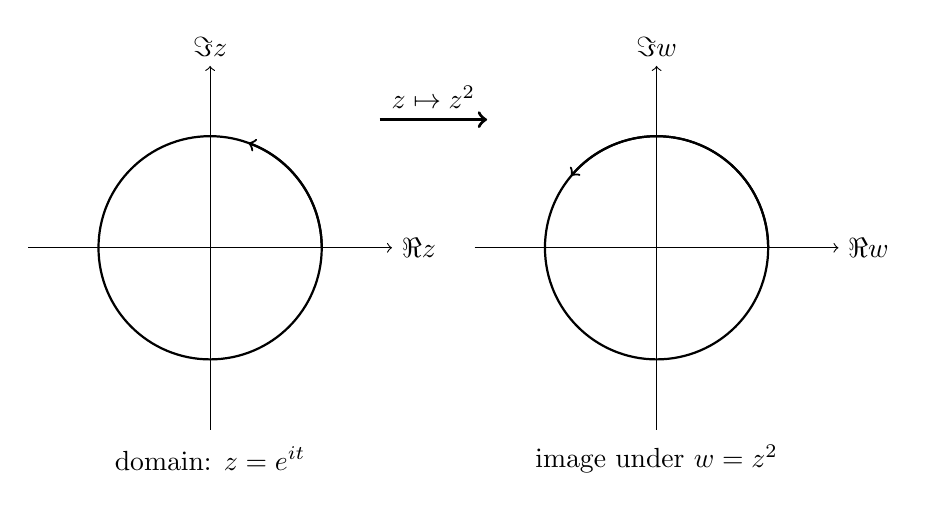
\begin{tikzpicture}[scale=1.05]
    \draw[->] (-2.2,0)--(2.2,0) node[right] {$\Re z$};
    \draw[->] (0,-2.2)--(0,2.2) node[above] {$\Im z$};
    \draw[thick] (0,0) circle (1.35);
    \draw[->,thick] (1.35,0) arc (0:70:1.35);
    \node at (0,-2.55) {domain: $z=e^{it}$};

    \begin{scope}[xshift=5.4cm]
    \draw[->] (-2.2,0)--(2.2,0) node[right] {$\Re w$};
    \draw[->] (0,-2.2)--(0,2.2) node[above] {$\Im w$};
    \draw[thick] (0,0) circle (1.35);
    \draw[->,thick] (1.35,0) arc (0:140:1.35);
    \node at (0,-2.55) {image under $w=z^2$};
    \end{scope}
    \draw[->,very thick] (2.05,1.55)--(3.35,1.55) node[midway,above] {$z\mapsto z^2$};
\end{tikzpicture}
\caption{The map $z\mapsto z^2$ doubles arguments. One traversal of an arc in the $z$-plane produces twice the angular change in the $w$-plane.}
\end{figure}

\begin{figure}[H]
\centering
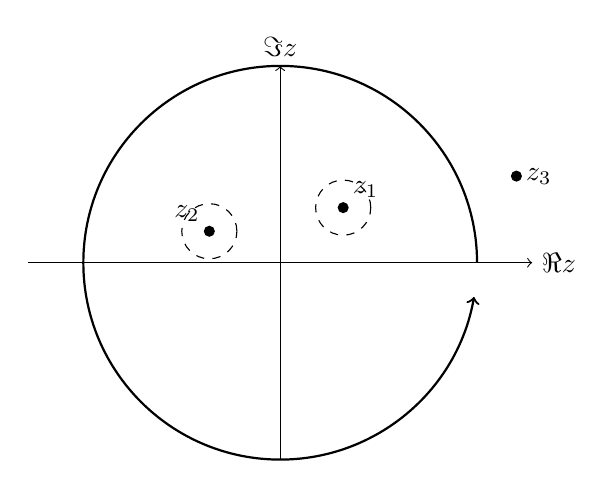
\begin{tikzpicture}[scale=1.0]
    \draw[->] (-3.2,0)--(3.2,0) node[right] {$\Re z$};
    \draw[->] (0,-2.5)--(0,2.5) node[above] {$\Im z$};
    \draw[thick,->] (2.5,0) arc (0:350:2.5);
    \fill (0.8,0.7) circle (2pt) node[above right] {$z_1$};
    \fill (-0.9,0.4) circle (2pt) node[above left] {$z_2$};
    \fill (3.0,1.1) circle (2pt) node[right] {$z_3$};
    \draw[dashed] (0.8,0.7) circle (0.35);
    \draw[dashed] (-0.9,0.4) circle (0.35);
\end{tikzpicture}
\caption{A residue contour encloses $z_1$ and $z_2$ but not $z_3$. The contour integral is $2\pi i$ times the sum of the enclosed residues, with winding numbers included.}
\end{figure}

\begin{remark}
The first picture encodes conformality: near a point where $f'(z_0)\neq0$, small directions are rotated by $\arg f'(z_0)$ and scaled by $|f'(z_0)|$. The second picture encodes locality of residues: the global contour integral is assembled from data in arbitrarily small neighborhoods of the enclosed singularities.
\end{remark}

\section{Conclusion}

Complex analysis begins with a small change in the definition of derivative: the increment $h$ is allowed to approach $0$ from every direction in the complex plane. This small change creates an extremely rigid theory. Holomorphic functions satisfy the Cauchy-Riemann equations, admit contour integral formulas, possess power series expansions, and have isolated singularities whose behavior is encoded by Laurent series.

The residue theorem is the computational climax of the elementary theory. It converts difficult contour integrals into algebraic data: the coefficients of $(z-z_0)^{-1}$ in local Laurent expansions. Conceptually, complex analysis shows how algebra, geometry, topology, and analysis become inseparable once the real line is replaced by the complex plane.
